% IEEE Conference/Journal Style LaTeX Document
% For use with Overleaf - https://www.overleaf.com
% ============================================

\documentclass[conference]{IEEEtran}

% ============================================
% PACKAGES
% ============================================
\usepackage[utf8]{inputenc}
\usepackage[T1]{fontenc}
\usepackage{graphicx}
\usepackage{hyperref}
\usepackage{booktabs}
\usepackage{array}
\usepackage{caption}
\usepackage{subcaption}
\usepackage{xcolor}
\usepackage{listings}
\usepackage{float}

% TODO note styling - elegant blue boxes
\newcommand{\todo}[1]{\textcolor{blue}{\small\textit{(To be completed: #1)}}}

% Hyperlink styling
\hypersetup{
    colorlinks=true,
    linkcolor=blue,
    filecolor=magenta,      
    urlcolor=cyan,
    citecolor=blue,
    pdftitle={The Hero in Four Worlds - AI Visual Storytelling},
    pdfauthor={UPT Student}
}

% Code listing style for prompts
\lstdefinestyle{promptstyle}{
    backgroundcolor=\color{gray!10},
    basicstyle=\ttfamily\footnotesize,
    breaklines=true,
    frame=single,
    framerule=0pt,
    xleftmargin=0.5em,
    xrightmargin=0.5em
}

% ============================================
% DOCUMENT START
% ============================================
\begin{document}

% ============================================
% TITLE
% ============================================
\title{The Hero in Four Worlds:\\AI-Powered Visual Storytelling with Consistent Character Design}

\author{
    \IEEEauthorblockN{[Your Name]}
    \IEEEauthorblockA{
        Master's Program: [Your Specialization]\\
        Politehnica University Timișoara\\
        Course: Graphics Processing Systems\\
        Supervisor: As.Drd.Ing. Bianca Gușiță\\
        January 2026
    }
}

\maketitle

% ============================================
% ABSTRACT
% ============================================
\begin{abstract}
This project explores the creative potential of modern AI image generation tools through the theme ``The Hero in Four Worlds'' — placing a consistent character across four dramatically different environments: a tropical jungle, a medieval town, a futuristic city, and a desert landscape. Using a combination of Seedream 4.5 \cite{seedream}, Nano Banana \cite{nanobanana}, and Flux Kontext \cite{fluxkontext}, we demonstrate a practical workflow for generating visually cohesive narratives while maintaining character consistency. The project evaluates each tool's strengths and weaknesses in terms of image quality, generation speed, creative flexibility, and consistency preservation. Results show that combining multiple specialized AI tools produces superior outcomes compared to using a single tool, with each platform excelling at different stages of the creative pipeline.
\end{abstract}

% ============================================
% KEYWORDS
% ============================================
\begin{IEEEkeywords}
AI image generation, character consistency, visual storytelling, Seedream, Nano Banana, Flux Kontext, generative AI
\end{IEEEkeywords}

% ============================================
% 1. INTRODUCTION
% ============================================
\section{Introduction}

\subsection{Project Theme}

This project explores the theme \textbf{``The Hero in Four Worlds''} — creating a consistent character placed across four dramatically different environments:

\begin{enumerate}
    \item \textbf{Jungle} — Dense tropical vegetation, wildlife, natural lighting
    \item \textbf{Medieval Town} — Historical architecture, cobblestone streets, period-appropriate atmosphere
    \item \textbf{Futuristic City} — Neon lights, advanced technology, cyberpunk aesthetics
    \item \textbf{Desert} — Arid landscape, harsh sunlight, sand dunes and oasis
\end{enumerate}

\subsection{Purpose of the Project}

This theme was chosen to test the capabilities of modern AI image generation tools in maintaining character consistency across vastly different environmental contexts. The challenge lies in placing the same hero character in four visually distinct worlds while preserving their identity, clothing, and features. This project demonstrates the practical workflow of combining multiple AI tools for creative visual storytelling.

\subsection{Objectives}

The primary objectives of this project are:

\begin{itemize}
    \item Generate 4 distinct world environment landscapes using AI tools
    \item Generate a consistent hero character design using AI image generation tools
    \item Place the character in 4 distinct world environments (7-10 total images)
    \item Evaluate and compare the performance of Seedream 4.5, Nano Banana, and Flux Kontext
    \item Document the creative workflow and analyze tool strengths/weaknesses
    \item Create a compelling visual narrative across all four worlds
\end{itemize}

% ============================================
% 2. TOOLS OVERVIEW
% ============================================
\section{Tools Overview}

This section describes the AI tools used in this project, their capabilities, and their specific roles in the creative workflow.

\subsection{Seedream 4.5 (ByteDance)}

\textbf{Official Website:} \url{https://seed.bytedance.com/en/seedream4_0}\\
\textbf{Access Platform:} \url{https://lovart.ai} (Seedream 4.5 integration) \cite{lovart}

\subsubsection{Description}
Seedream 4.5 is ByteDance's advanced AI image generation model, known for producing high-resolution, photorealistic images with excellent detail and composition. It excels at generating complex scenes with multiple elements, dramatic lighting, and cinematic compositions. The model responds well to structured prompts following the formula: Subject + Environment + Style + Technical Specs.

\subsubsection{Role in Project}
Used as the primary tool for generating all four world landscape backgrounds (Jungle, Desert, Medieval Town, Futuristic City). Seedream 4.5 was chosen for its ability to create detailed, high-resolution environments in 16:9 landscape format suitable for desktop wallpaper quality.

\subsection{Nano Banana}

\textbf{Website:} \url{https://nanobanana.ai/}

\subsubsection{Description}
Nano Banana is an AI-powered image editing platform specialized in maintaining character and object consistency across multiple images. It allows users to upload reference images and seamlessly insert consistent elements into new scenes.

\subsubsection{Role in Project}
Used for inserting the hero character into all four world landscapes while maintaining consistent appearance, clothing, and features across different environments. \todo{Update after using the tool}

\subsection{Flux Kontext}

\textbf{Website:} \url{https://flux-context.org/}

\subsubsection{Description}
Flux Kontext is a context-aware AI image editing tool that excels at making local, targeted edits to images while preserving the overall composition. It is particularly useful for fine adjustments, background modifications, and adding/removing specific details.

\subsubsection{Role in Project}
Used for final polish and context-aware edits such as lighting adjustments, adding environmental details, and fixing any artifacts from the character insertion process. \todo{Update after using the tool}

\subsection{Additional Tools}

\textbf{lovart.ai} — Web platform providing access to Seedream 4.5 with a user-friendly interface. Used as the primary access point for Seedream due to its intuitive controls and aspect ratio settings.

% ============================================
% 3. METHODOLOGY
% ============================================
\section{Methodology}

\subsection{Workflow Overview}

The project follows a three-phase approach: first generating all world landscapes, then creating a consistent hero character, and finally compositing the character into each world with refinements.

\begin{figure}[H]
\centering
\fbox{
\begin{minipage}{0.9\linewidth}
\centering
\texttt{SEEDREAM 4.5} $\rightarrow$ \texttt{NANO BANANA} $\rightarrow$ \texttt{FLUX KONTEXT}\\[0.5em]
\small{World Landscapes} \hspace{1em} \small{Hero Insertion} \hspace{1em} \small{Final Polish}
\end{minipage}
}
\caption{Three-phase workflow diagram}
\label{fig:workflow}
\end{figure}

\textbf{Phase 1:} Generate all four world landscapes with designated ``hero spots'' — areas where the character will be placed later (stone pedestal in jungle, empty camel saddle in desert, etc.)

\textbf{Phase 2:} Create the hero character reference and use Nano Banana to insert them consistently into each landscape.

\textbf{Phase 3:} Use Flux Kontext for final adjustments, lighting fixes, and detail enhancement.

\subsection{Order of Tools Used}

Table~\ref{tab:toolorder} shows the sequential order in which tools were applied throughout the project.

\begin{table}[H]
\centering
\caption{Tool Usage Order}
\label{tab:toolorder}
\begin{tabular}{|c|l|p{5cm}|}
\hline
\textbf{Step} & \textbf{Tool} & \textbf{Purpose} \\
\hline
1 & Seedream 4.5 & Generate 4 world landscape backgrounds \\
2 & Seedream 4.5 & Create hero character reference image \\
3 & Nano Banana & Insert hero with consistency across scenes \\
4 & Flux Kontext & Final polish and detail adjustments \\
\hline
\end{tabular}
\end{table}

\subsection{Prompts Used}

This section documents the prompts used for each generation, following the Seedream 4.5 best practices: Subject + Environment + Style + Technical Specs.

\subsubsection{Hero Character Reference Prompt}

The hero character was designed as a consistent reference sheet showing multiple angles for use with Nano Banana's character insertion capabilities. Table~\ref{tab:herotraits} summarizes the distinctive character traits.

\begin{table}[H]
\centering
\caption{Hero Character Traits}
\label{tab:herotraits}
\begin{tabular}{|l|p{6cm}|}
\hline
\textbf{Attribute} & \textbf{Description} \\
\hline
Inspiration & Timoth\'{e}e Chalamet \\
Age & 20-25 years old \\
Build & Athletic lean, approx. 180cm \\
Face & Sharp jawline, high cheekbones \\
Eyes & Deep-set, hazel-green, expressive \\
Eyebrows & Thick, dark, natural arch \\
Nose & Straight, refined \\
Hair & Dark brown-black, slicked back \\
Facial Hair & Well-groomed short goatee \\
Skin & Medium tone, warm undertones \\
Tattoo & Visible on right forehand \\
Accessory & Black ring on left index finger \\
Expression & Intense, confident gaze \\
\hline
\end{tabular}
\end{table}

\begin{lstlisting}[style=promptstyle]
Character reference sheet of a handsome young man age 20-25, Timothee Chalamet inspired features, DISTINCTIVE FACE with sharp defined jawline, high prominent cheekbones, deep-set expressive hazel-green eyes, thick dark eyebrows with natural arch, straight refined nose, full lips, medium skin tone with subtle warm undertones, dark brown-black slightly longer hair slicked back, well-groomed short goatee, visible tattoo on his right forehand, athletic lean build not overly muscular approximately 180cm tall, black ring on the left hand's index finger, intense confident gaze, wearing simple neutral gray t-shirt and pants, showing FRONT VIEW, SIDE VIEW, THREE-QUARTER VIEW, and BACK VIEW arranged in a row, character turnaround sheet, full body poses, clean white background, consistent lighting across all angles, photorealistic, 4K resolution, highly detailed facial features for character consistency, professional character design reference sheet
\end{lstlisting}

\begin{figure}[H]
\centering
\includegraphics[width=0.95\linewidth]{images/hero_reference.png}
\caption{Hero character reference sheet showing front, side, 3/4, and back views for consistency. Generated with Seedream 4.5 via lovart.ai.}
\label{fig:hero}
\end{figure}

\subsubsection{Jungle World Prompt}

\begin{lstlisting}[style=promptstyle]
Dense tropical jungle, lush green canopy with towering ancient trees, golden sunbeams piercing through the foliage creating god rays, volumetric lighting, a prominent mossy stone plateau in the center of a clearing bathed in sunlight, a majestic lion sitting beside the stone looking upward toward the top of the stone with curious attention, colorful parrots perched on branches, monkeys in the trees, a toucan with vibrant beak, butterflies floating in the light beams, misty atmosphere, rich vegetation with ferns and exotic flowers, wide panoramic view, landscape orientation, cinematic widescreen composition, photorealistic, 16:9 aspect ratio, 4K resolution, highly detailed
\end{lstlisting}

\subsubsection{Desert World Prompt}

\begin{lstlisting}[style=promptstyle]
Vast golden desert landscape at warm afternoon light, endless rolling sand dunes stretching to the horizon, gentle wind lifting wisps of sand into the air, delicate sand particles drifting across the scene, a shimmering oasis with palm trees visible in the far distance, a caravan of camels with riders traveling in the background slightly out of focus, in the foreground center a single majestic camel with ornate saddle and decorative blankets standing ready with no rider, the camel's mane and saddle fabric gently blowing in the breeze, soft desert haze, heat shimmer effect, dramatic shadows on dunes, wide panoramic view, landscape orientation, cinematic composition, 16:9 aspect ratio, 4K resolution, photorealistic, National Geographic style
\end{lstlisting}

\subsubsection{Medieval Town Prompt}

\begin{lstlisting}[style=promptstyle]
Epic medieval jousting tournament at golden hour, grand arena with colorful heraldic banners, in the foreground center a magnificent white warhorse with ornate saddle FACING DIRECTLY TOWARD THE CAMERA with NO RIDER ready for its champion, the horse standing proud and battle-ready, behind it at the far end of the arena an opponent knight in dark armor mounted on a black horse FACING AWAY with back toward camera preparing to charge, a beautiful princess in elegant gown watching from an ornate royal balcony waving a silk favor, crowds cheering from wooden stands, king and nobles in the royal box, dramatic tension before the joust, wide panoramic view, landscape orientation, photorealistic, 16:9 aspect ratio, 4K resolution, cinematic medieval fantasy
\end{lstlisting}

\subsubsection{Futuristic City Prompt}

\begin{lstlisting}[style=promptstyle]
Breathtaking cyberpunk rooftop vista at night, standing at the edge of a rain-soaked skyscraper overlooking Night City, thousands of neon lights illuminating the urban canyon below, aerodynes and flying cars zooming between massive holographic billboards, cherry blossom petals drifting in the wind mixing with rain, empty rooftop ledge in foreground center, towering corporate arcologies piercing the smog layer, flickering advertisements, steam rising from vents, Cyberpunk 2077 and Blade Runner 2049 aesthetic, ultra-wide cinematic composition, landscape orientation, 16:9 aspect ratio, 4K resolution, photorealistic, dramatic mood lighting, neon noir atmosphere
\end{lstlisting}

\subsection{Intermediate Results}

Table~\ref{tab:progress} shows the current progress of landscape generation.

\begin{table}[H]
\centering
\caption{Landscape Generation Progress}
\label{tab:progress}
\begin{tabular}{|l|c|l|p{3.5cm}|}
\hline
\textbf{World} & \textbf{Status} & \textbf{File} & \textbf{Hero Spot} \\
\hline
Jungle & Complete & jungle\_1.png & Stone plateau \\
Desert & Complete & desert\_1.png & Empty camel saddle \\
Medieval & Complete & medieval\_3.png & Riderless warhorse (facing camera) \\
Futuristic & Complete & cyberpunk\_1.png & Rooftop edge \\
\hline
\end{tabular}
\end{table}

% ============================================
% 4. RESULTS
% ============================================
\section{Results}

\subsection{Final Images}

\subsubsection{Jungle Landscape}

\begin{figure}[H]
\centering
\includegraphics[width=0.85\linewidth]{images/jungle_1.png}
\caption{Jungle world landscape with stone plateau and lion. Generated with Seedream 4.5 via lovart.ai.}
\label{fig:jungle}
\end{figure}

\textbf{World:} Jungle\\
\textbf{Tool(s) Used:} Seedream 4.5 (lovart.ai)\\
\textbf{Description:} Dense tropical jungle scene featuring golden sunbeams piercing through the canopy, creating dramatic god rays. A mossy stone plateau in the center serves as the designated hero spot. A lion sits beside the stone, gazing upward, creating a natural focal point for where the hero will stand.

\subsubsection{Desert Landscape}

\begin{figure}[H]
\centering
\includegraphics[width=0.85\linewidth]{images/desert_1.png}
\caption{Desert world landscape with camel and distant oasis. Generated with Seedream 4.5 via lovart.ai.}
\label{fig:desert}
\end{figure}

\textbf{World:} Desert\\
\textbf{Tool(s) Used:} Seedream 4.5 (lovart.ai)\\
\textbf{Description} Vast golden desert with rolling sand dunes, an oasis visible in the distance, and a caravan in the background. A single camel with ornate saddle stands ready in the foreground — the empty saddle serves as the hero spot where the character will be placed.

\subsubsection{Medieval Town}

\begin{figure}[H]
\centering
\includegraphics[width=0.85\linewidth]{images/medieval_3.png}
\caption{Medieval jousting tournament with riderless warhorse facing camera, opponent knight with back to viewer, and princess on balcony. Generated with Seedream 4.5 via lovart.ai.}
\label{fig:medieval}
\end{figure}

\textbf{World:} Medieval Town\\
\textbf{Tool(s) Used:} Seedream 4.5 (lovart.ai)\\
\textbf{Description:} Epic jousting tournament with reversed composition — the hero's white warhorse faces directly toward the camera while the opponent knight has his back to the viewer. This setup allows for front-facing hero insertion.

\subsubsection{Futuristic City}

\begin{figure}[H]
\centering
\includegraphics[width=0.85\linewidth]{images/cyberpunk_1.png}
\caption{Cyberpunk rooftop overlooking neon-lit megacity with flying vehicles. Generated with Seedream 4.5 via lovart.ai.}
\label{fig:futuristic}
\end{figure}

\textbf{World:} Futuristic City\\
\textbf{Tool(s) Used:} Seedream 4.5 (lovart.ai)\\
\textbf{Description:} Breathtaking cyberpunk rooftop vista at night overlooking a neon-lit megacity. Flying vehicles zoom between holographic billboards while rain and cherry blossoms drift through the air. The empty rooftop ledge in the foreground serves as the hero spot where the character will stand surveying the city.

\subsection{Hero Composites}

This section presents the final composited images where the hero character has been inserted into each landscape using Nano Banana.

\subsubsection{Desert — Hero Composite}

See Figure~\ref{fig:desert_hero}.

\noindent\textbf{Outfit:} Traditional white desert robes with headscarf (keffiyeh style)

\noindent\textbf{Pose:} Sitting on camel saddle, looking at camera

\noindent\textbf{Tool Used:} Nano Banana

\noindent\textbf{Observation:} Slight quality reduction observed during compositing compared to original Seedream 4.5 output.

\begin{figure}[H]
\centering
\includegraphics[width=0.85\linewidth]{images/hero_in_backgrounds/desert.png}
\caption{Hero character inserted into desert scene, wearing white desert robes and riding the camel. Composited using Nano Banana.}
\label{fig:desert_hero}
\end{figure}

\subsubsection{Jungle — Hero Composite}

See Figure~\ref{fig:jungle_hero}.

\noindent\textbf{Outfit:} Mowgli/Tarzan jungle style — minimal clothing, bare chest, loincloth

\noindent\textbf{Pose:} Standing heroically on stone plateau, commanding presence

\noindent\textbf{Tool Used:} Nano Banana

\noindent\textbf{Note:} May require Flux Kontext refinement for seamless integration.

\begin{figure}[H]
\centering
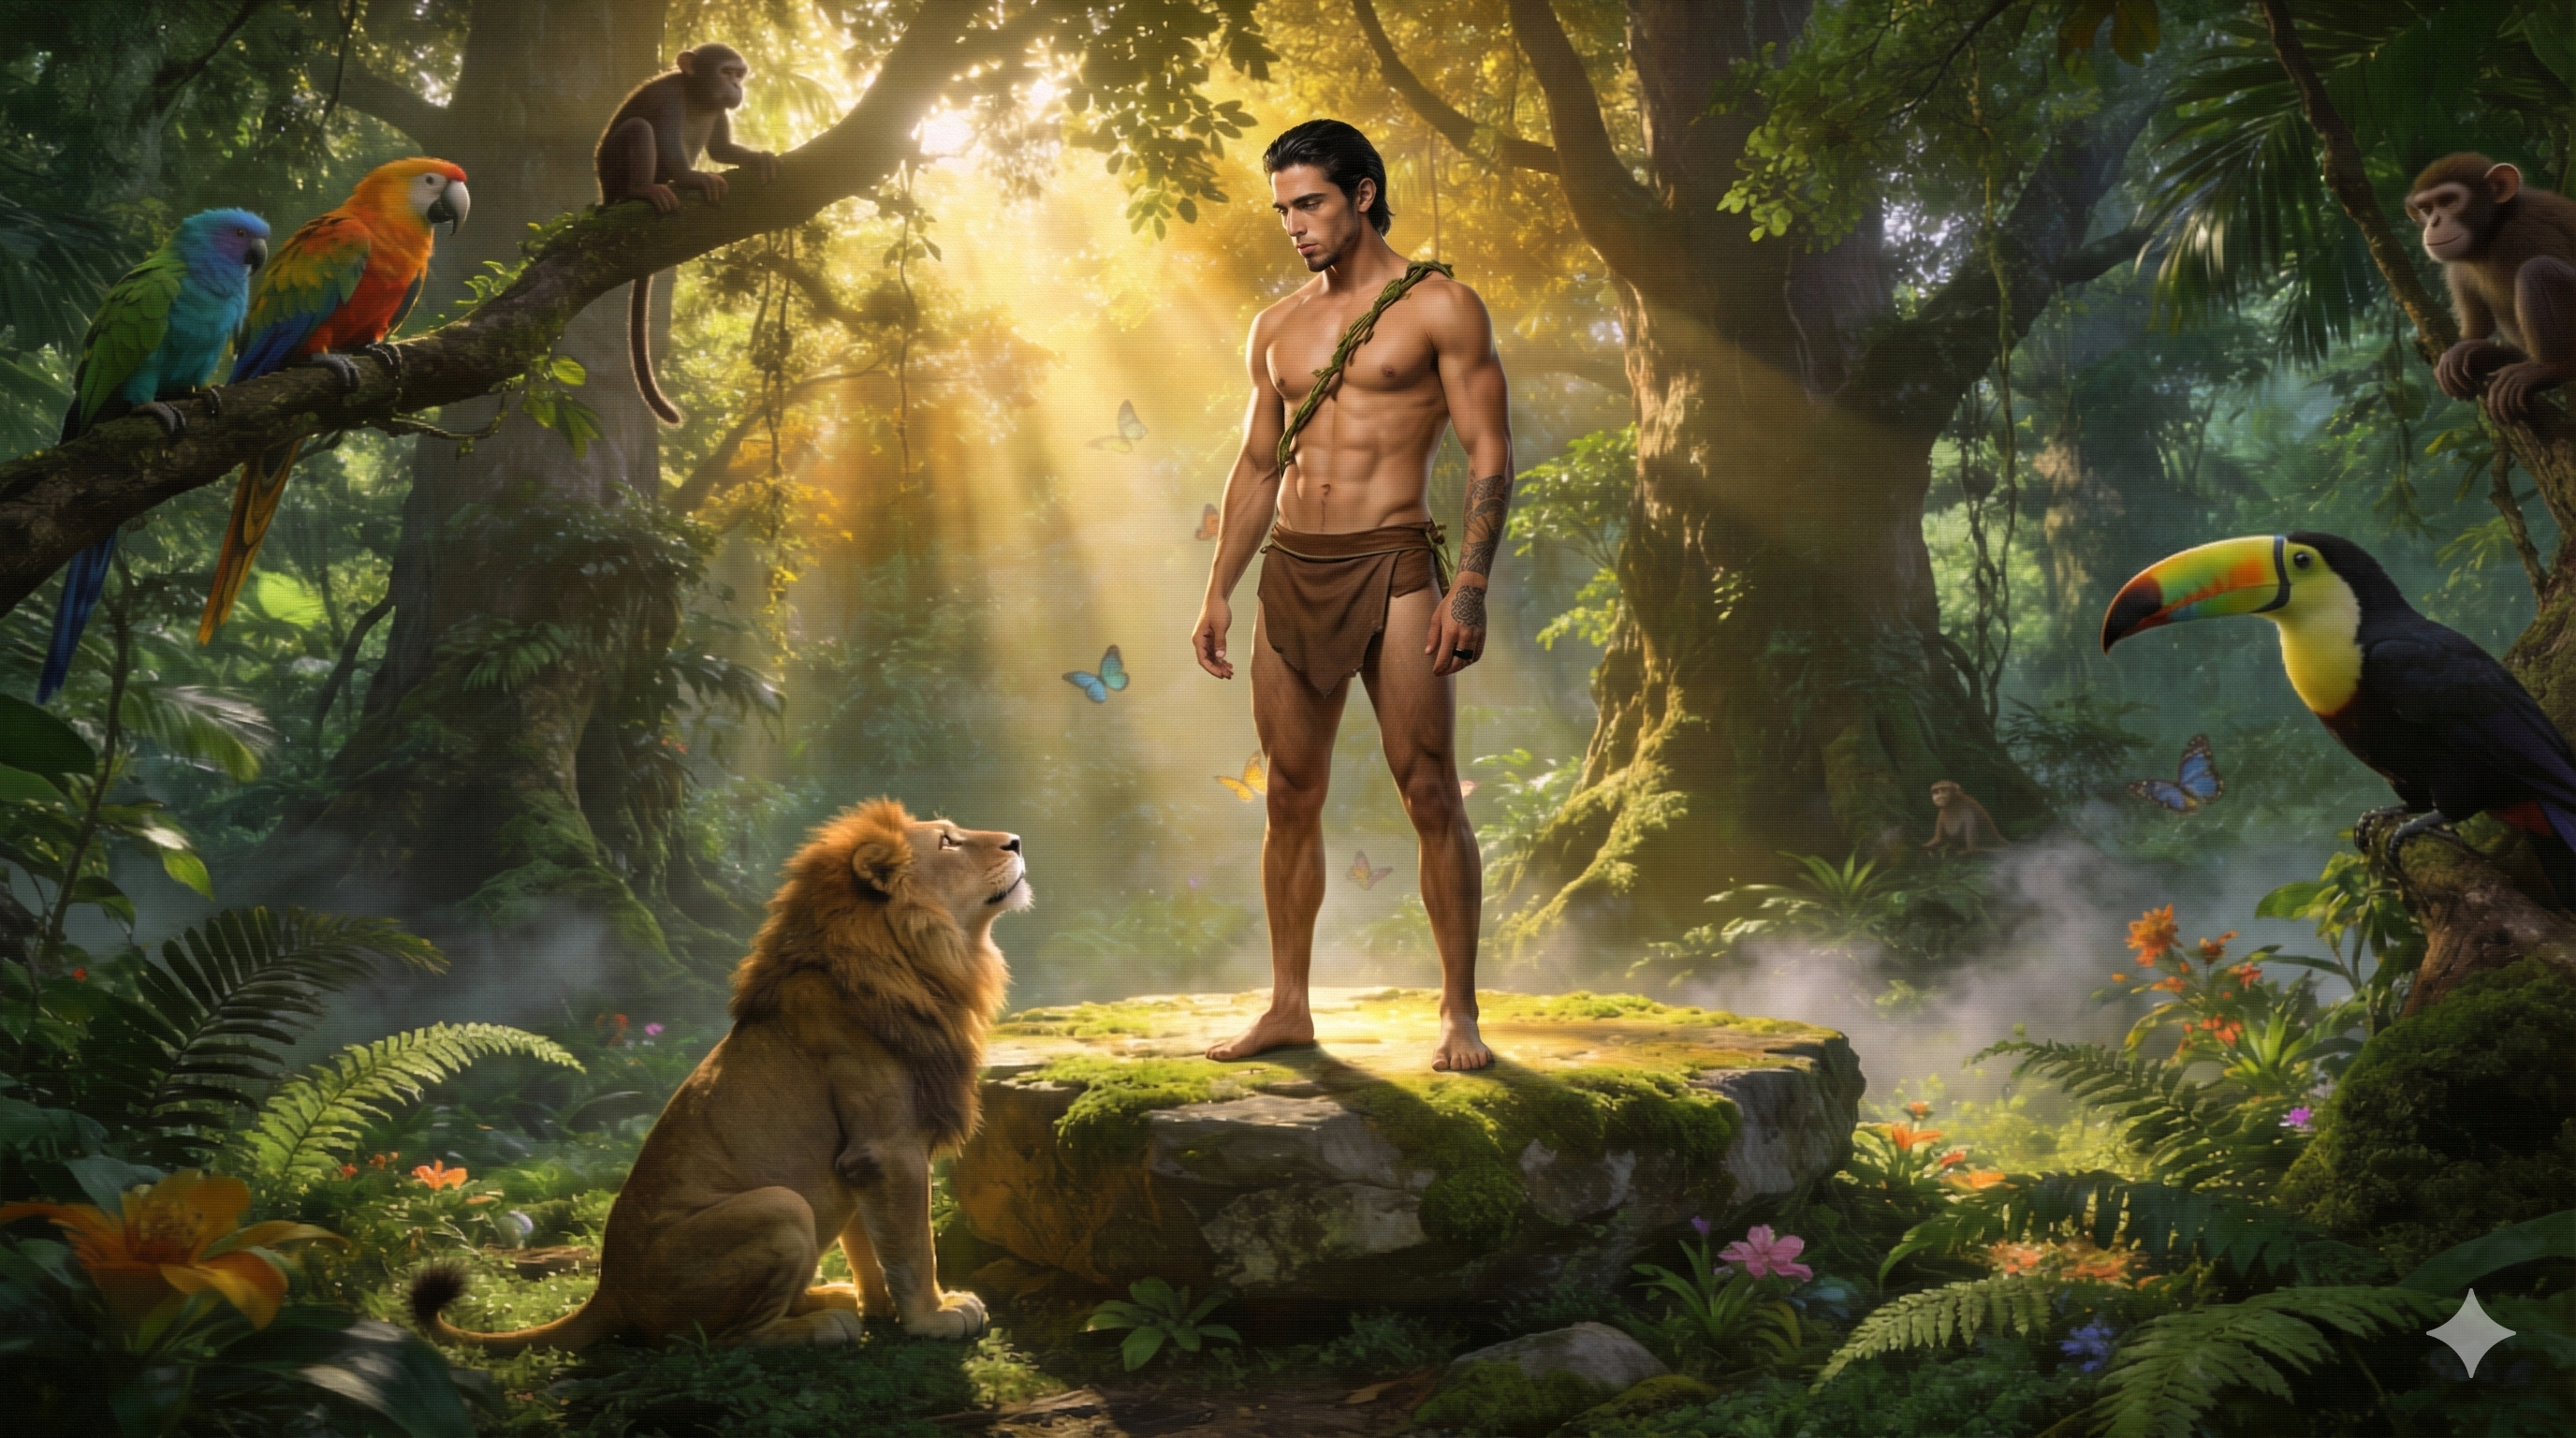
\includegraphics[width=0.85\linewidth]{images/hero_in_backgrounds/jungle.png}
\caption{Hero character as king of the jungle, standing on stone plateau in Mowgli/Tarzan style. Composited using Nano Banana.}
\label{fig:jungle_hero}
\end{figure}

\subsubsection{Medieval — Hero Composite}

See Figure~\ref{fig:medieval_hero}.

\noindent\textbf{Outfit:} Silver knight armor, no helmet (face and hair visible)

\noindent\textbf{Pose:} Mounted on warhorse facing camera, holding jousting lance, fierce expression

\noindent\textbf{Tool Used:} Nano Banana

\begin{figure}[H]
\centering
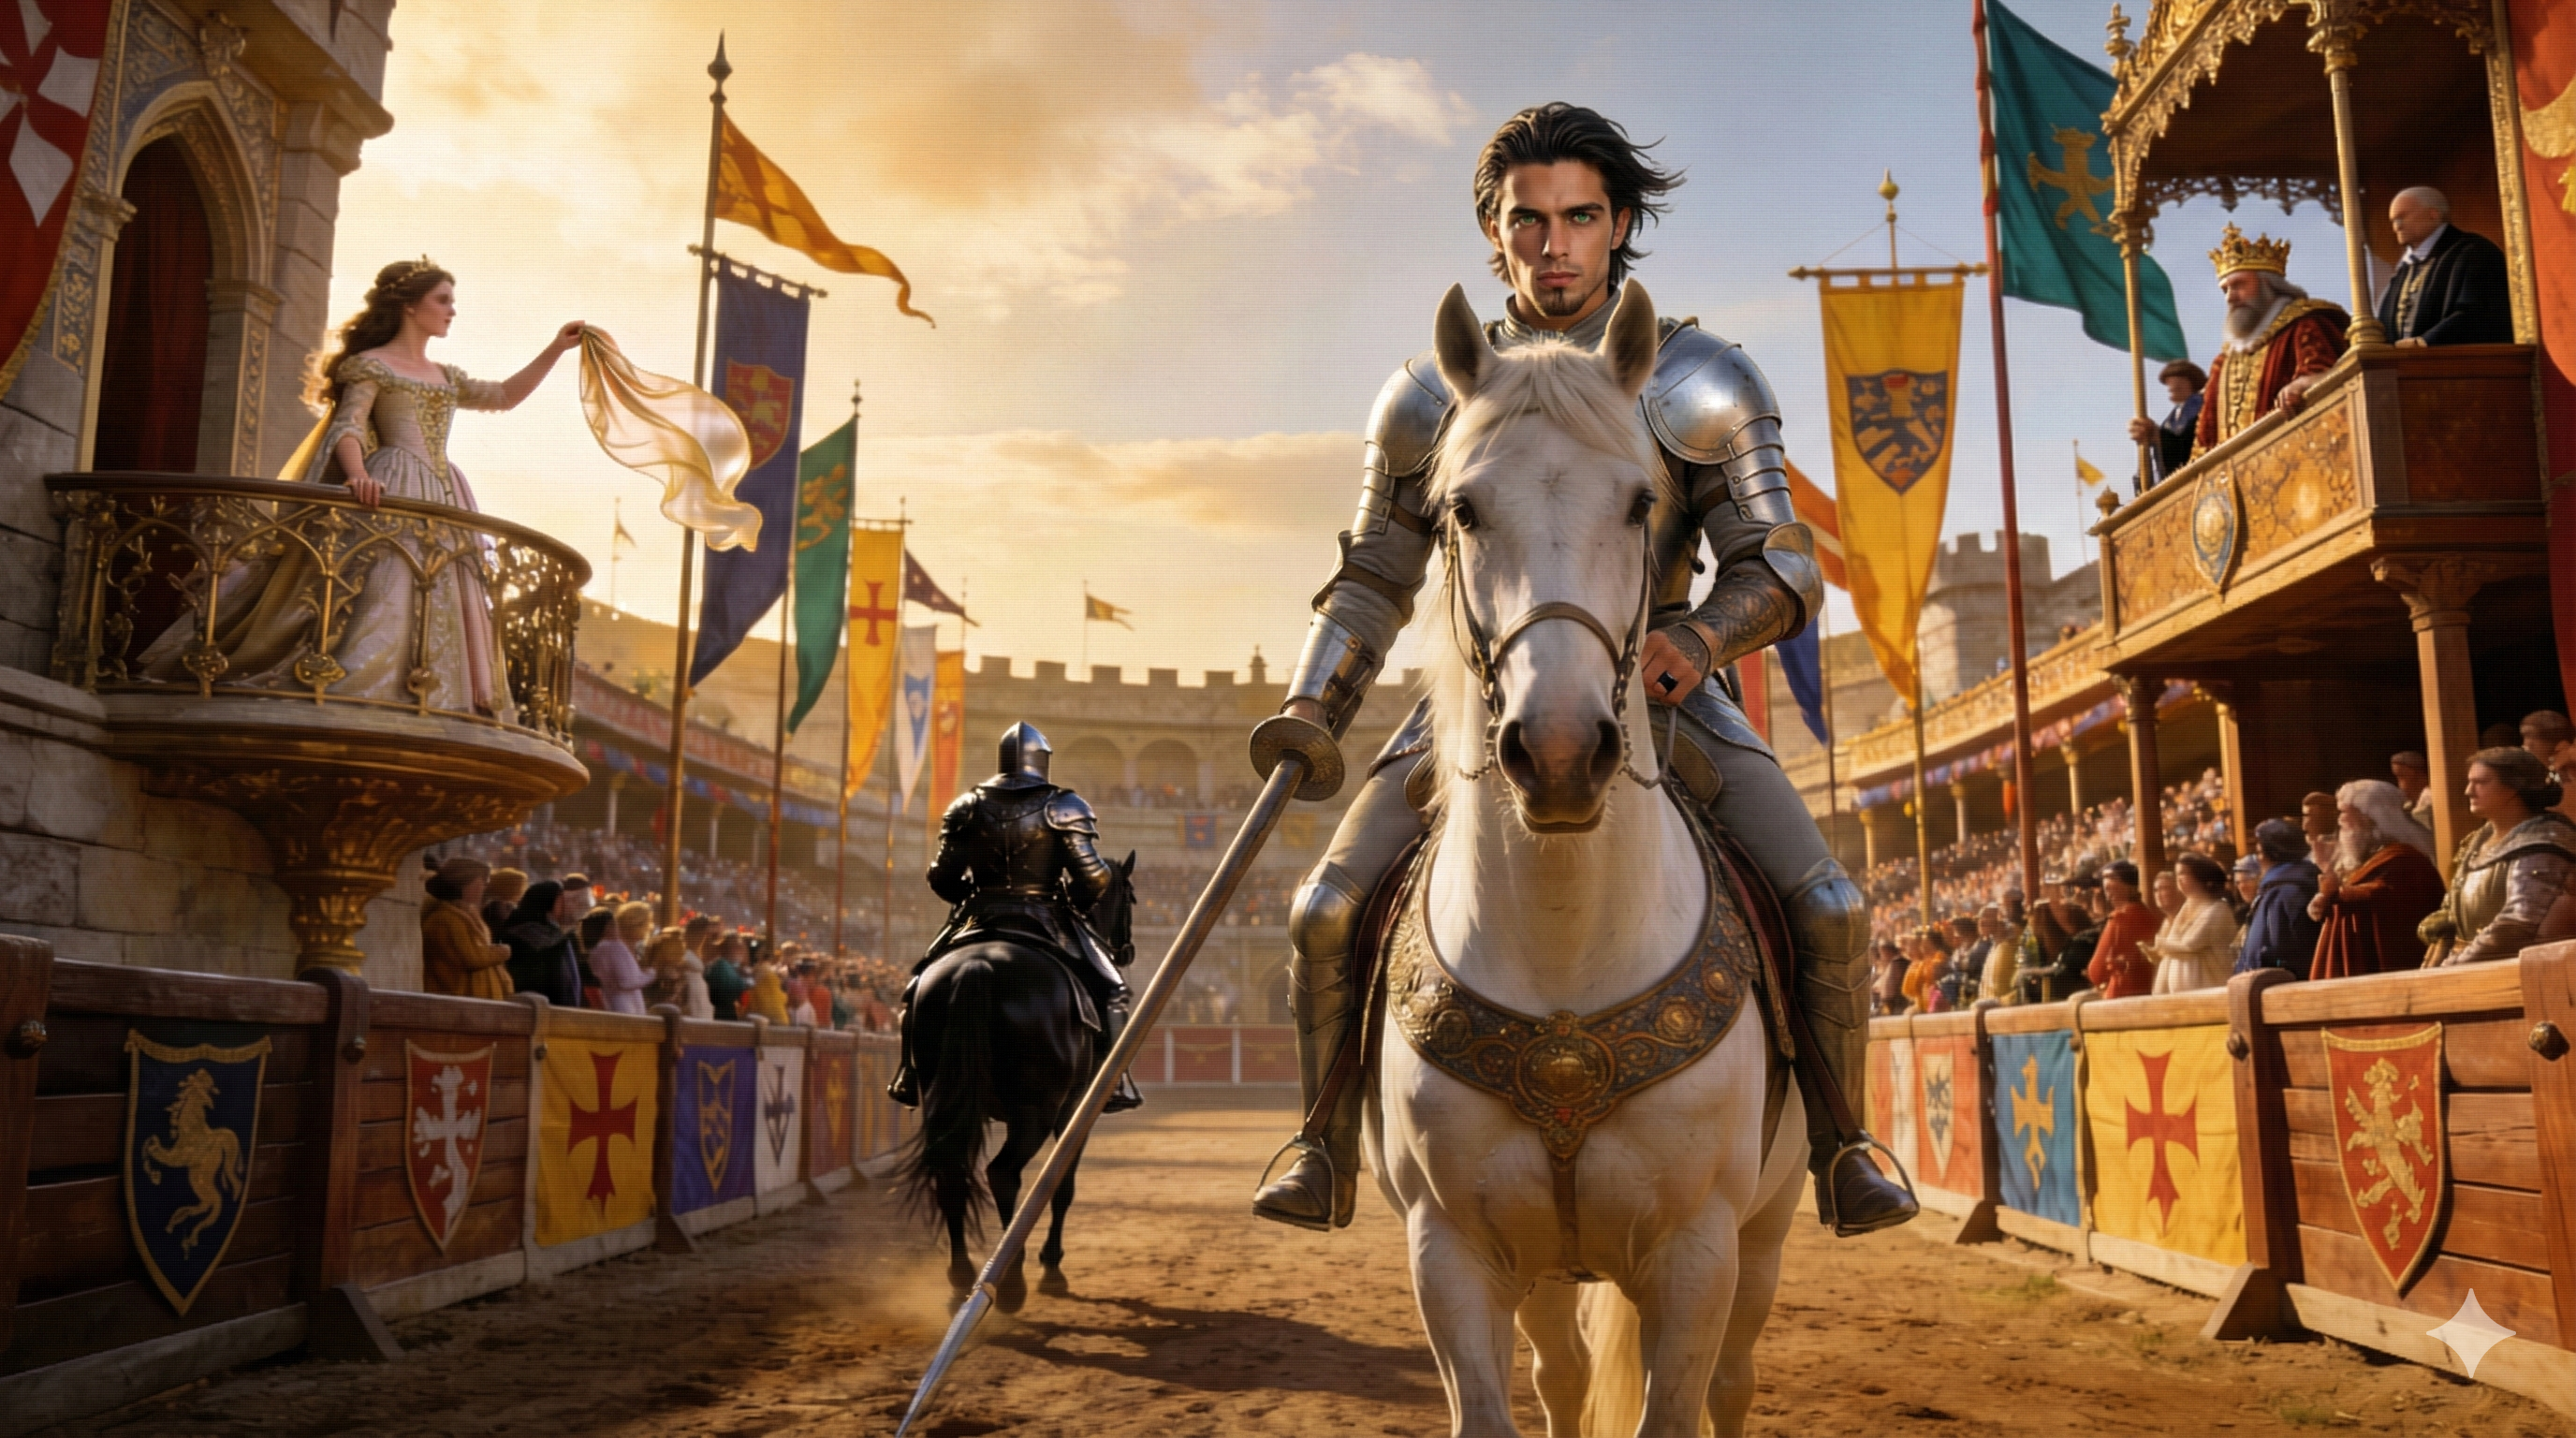
\includegraphics[width=0.85\linewidth]{images/hero_in_backgrounds/medieval.png}
\caption{Hero as knight mounted on warhorse facing camera, silver armor without helmet, ready for joust. Composited using Nano Banana.}
\label{fig:medieval_hero}
\end{figure}

\subsubsection{Cyberpunk — Hero Composite}

See Figure~\ref{fig:cyberpunk_hero}.

\noindent\textbf{Outfit:} Sleek black futuristic jacket with tech details, dark pants, combat boots

\noindent\textbf{Pose:} Standing at rooftop edge, looking over shoulder or gazing at city

\noindent\textbf{Tool Used:} Nano Banana

\noindent\textbf{Note:} Enhanced prompt used to maintain photorealistic quality and avoid stylized/drawn appearance.

\begin{figure}[H]
\centering
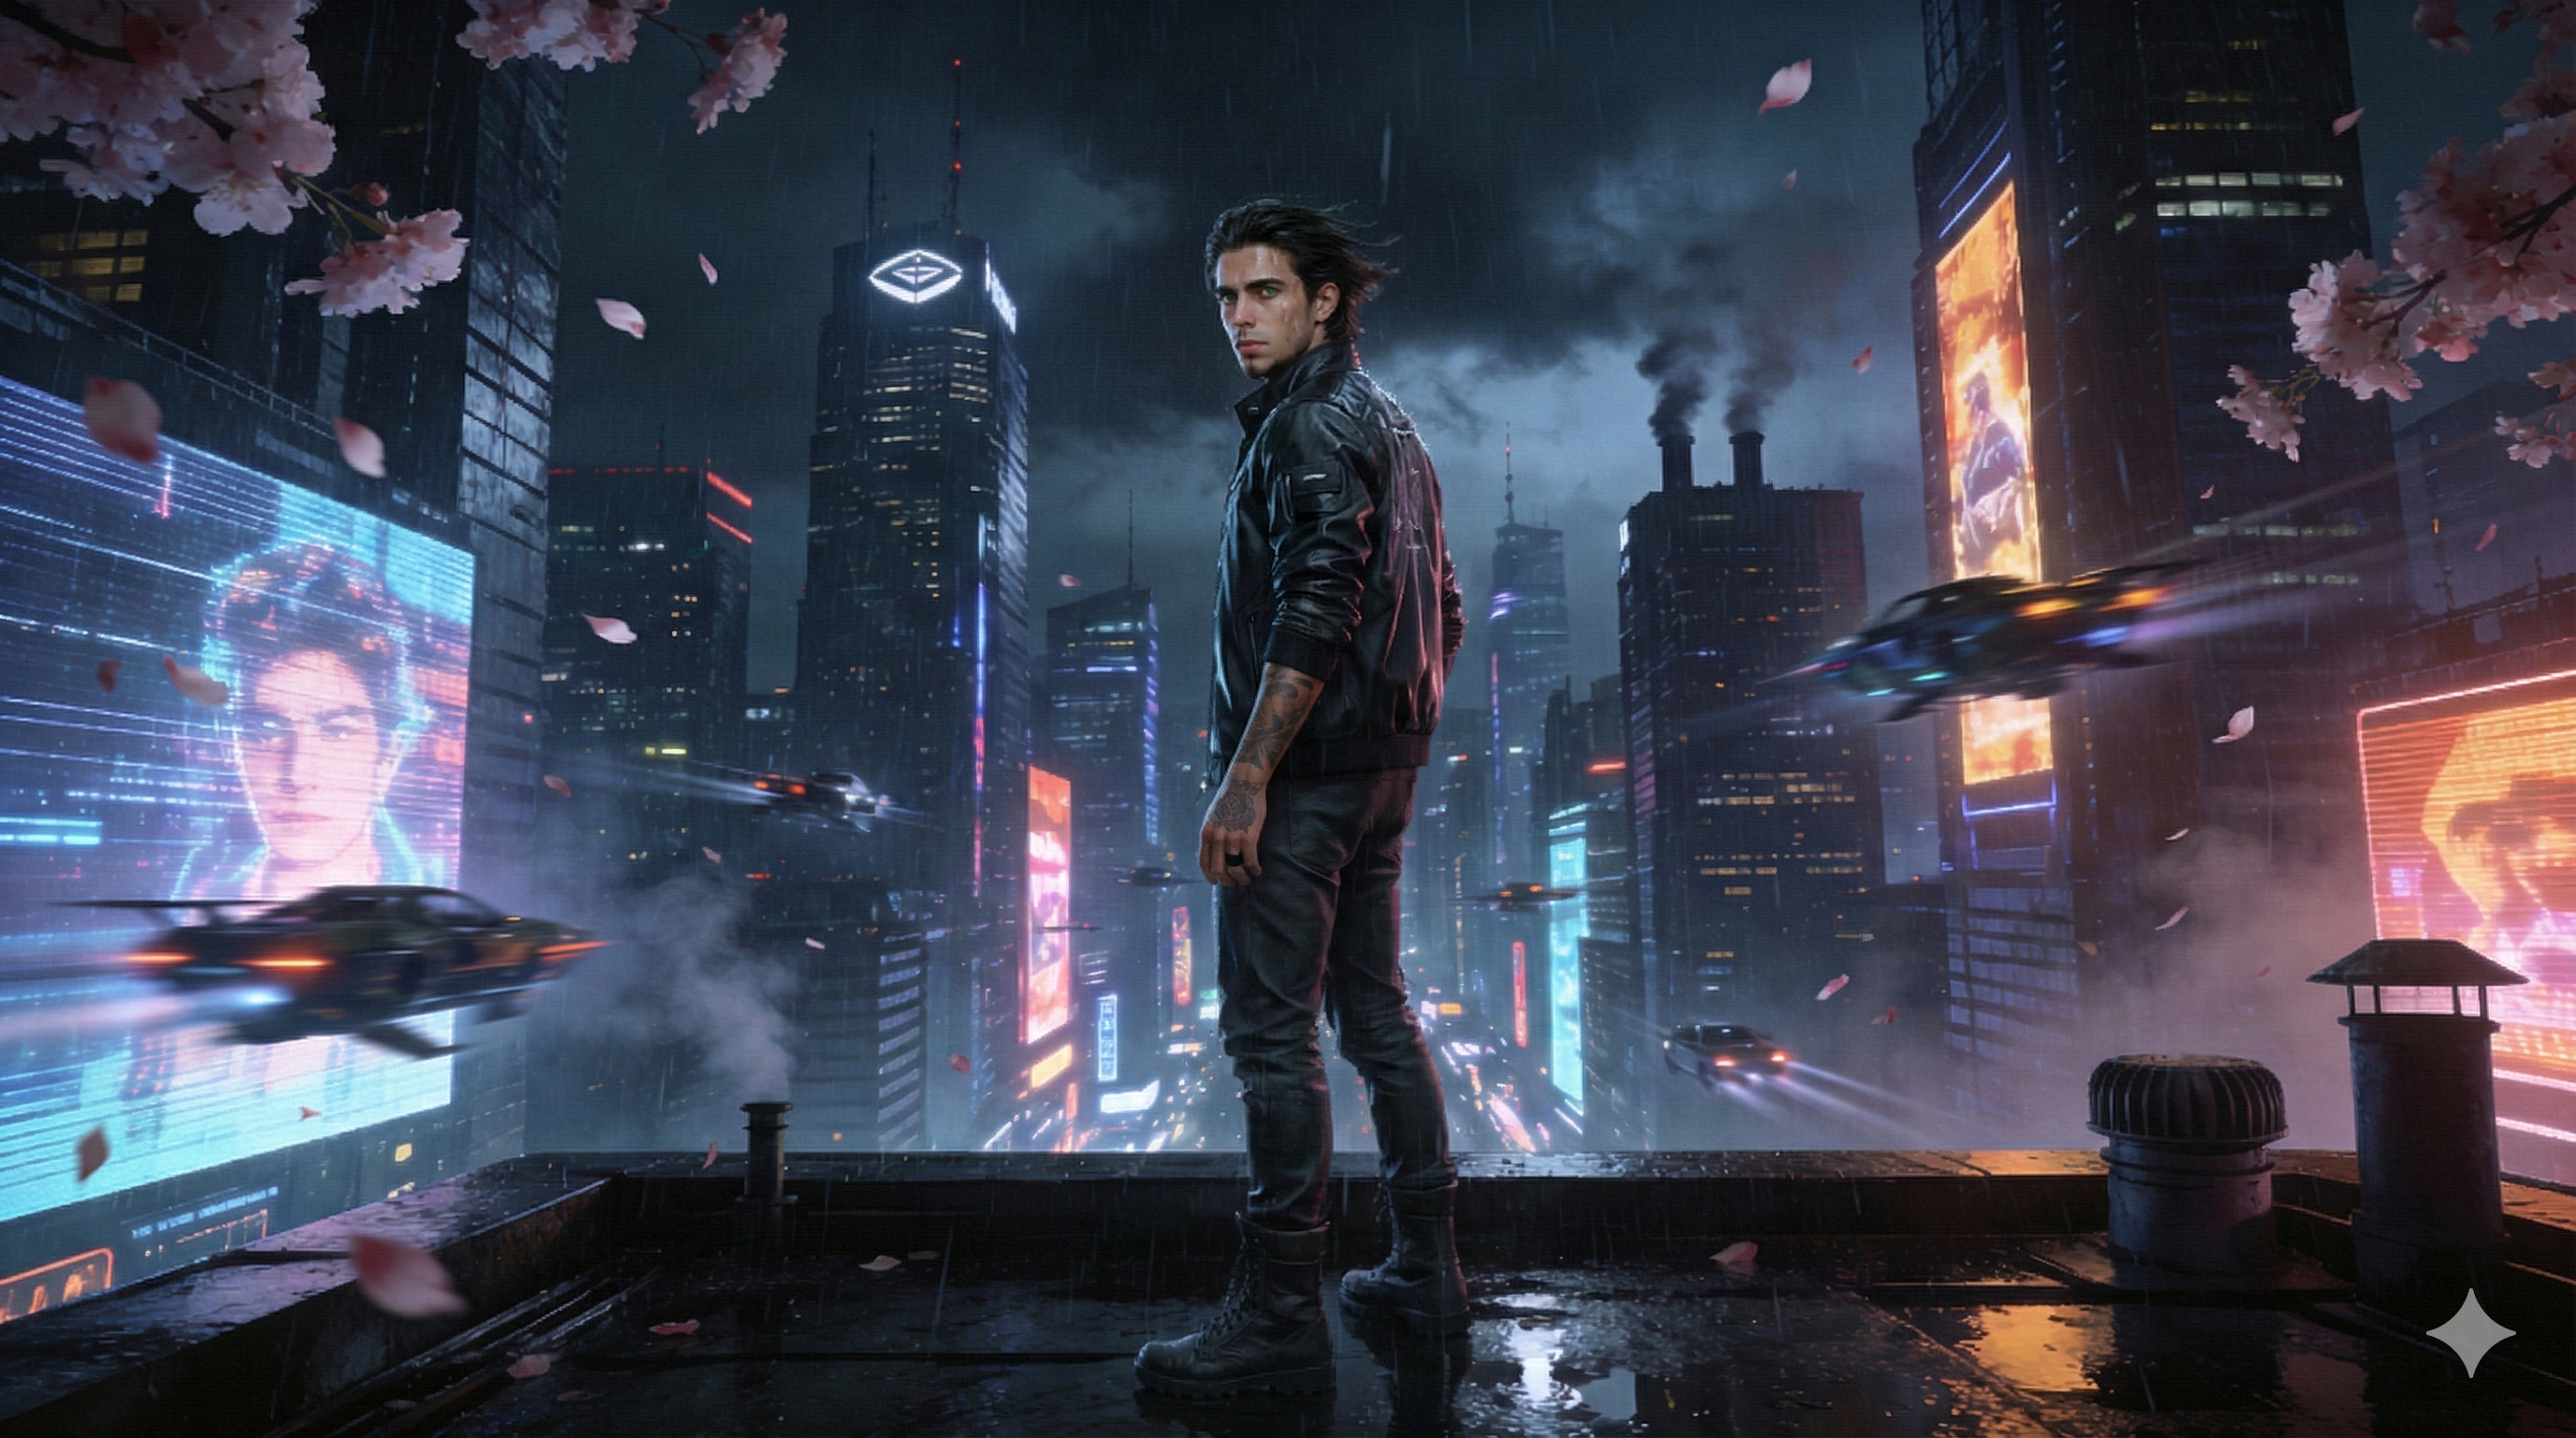
\includegraphics[width=0.85\linewidth]{images/hero_in_backgrounds/cyberpunk.png}
\caption{Hero in futuristic tech outfit standing at rooftop edge overlooking neon-lit city. Composited using Nano Banana.}
\label{fig:cyberpunk_hero}
\end{figure}

\subsection{In-Context Editing Comparison}

This section compares in-context editing capabilities between Flux-2 Pro and Nano Banana using the same prompt on the cyberpunk scene.

\subsubsection{Edit Prompt Used}

\begin{lstlisting}[style=promptstyle]
CRITICAL: DO NOT MODIFY THE CHARACTER'S APPEARANCE, FACE, BODY, CLOTHING, 
OR POSITION. Keep all character features EXACTLY as they are.
DO NOT change the background or city elements.

ONLY ADD: A holographic lion projection from the character's ring.

Character's left hand raised in front of him, palm facing up. 
From the BLACK RING on his left index finger, a glowing holographic 
LION is projected - a majestic blue-cyan hologram of a lion resembling 
the one from the jungle, made of translucent glowing light particles 
and geometric wireframe lines. The hologram lion is visible and prominent, 
floating above the ring, looking powerful and alert.

The hologram casts soft blue light on character's face and hand.
Futuristic AR tech visualization, cyberpunk aesthetic.

ONLY ADD the holographic lion element.
Photorealistic integration.
\end{lstlisting}

\subsubsection{Flux-2 Pro Result}

\begin{figure}[H]
\centering
\includegraphics[width=0.85\linewidth]{images/in-context-editing/flux-2/cyberpunk.jpg}
\caption{Cyberpunk scene with holographic lion edit using Flux-2 Pro.}
\label{fig:flux_edit}
\end{figure}

\textbf{Observations:} Resolution maintained at high quality. Hologram placement less intuitive but output remains crisp and detailed.

\subsubsection{Nano Banana Result}

\begin{figure}[H]
\centering
\includegraphics[width=0.85\linewidth]{images/in-context-editing/nano-banana/cyberpunk.png}
\caption{Cyberpunk scene with holographic lion edit using Nano Banana.}
\label{fig:nano_edit}
\end{figure}

\textbf{Observations:} Hologram positioning more logical and natural. However, some resolution/quality reduction observed compared to Flux-2 Pro output.

\subsubsection{Medieval Rearing Horse — Flux-2 Pro}

\begin{figure}[H]
\centering
\includegraphics[width=0.85\linewidth]{images/in-context-editing/flux-2/medieval.jpg}
\caption{Medieval scene with rearing horse edit using Flux-2 Pro.}
\label{fig:flux_medieval}
\end{figure}

\textbf{Observations:} Very crisp output with excellent lighting. Details remain sharp and on point. Overall superior quality preservation.

\subsubsection{Medieval Rearing Horse — Nano Banana}

\begin{figure}[H]
\centering
\includegraphics[width=0.85\linewidth]{images/in-context-editing/nano-banana/medieval.png}
\caption{Medieval scene with rearing horse edit using Nano Banana.}
\label{fig:nano_medieval}
\end{figure}

\textbf{Observations:} Slight cartoon-like stylization introduced. Quality dropped compared to Flux-2 Pro. Edit interpretation reasonable but less photorealistic.

\subsubsection{Jungle Ring Origin — Flux-2 Pro}

\begin{figure}[H]
\centering
\includegraphics[width=0.85\linewidth]{images/in-context-editing/flux-2/jungle.jpg}
\caption{Jungle scene with mystical ring origin edit using Flux-2 Pro.}
\label{fig:flux_jungle}
\end{figure}

\textbf{Observations:} More creative interpretation with additional creatures and excellent lighting effects. However, character has an extra arm artifact. With polishing, could work well. Overall more imaginative but less accurate.

\subsubsection{Jungle Ring Origin — Nano Banana}

\begin{figure}[H]
\centering
\includegraphics[width=0.85\linewidth]{images/in-context-editing/nano-banana/jungle.png}
\caption{Jungle scene with mystical ring origin edit using Nano Banana.}
\label{fig:nano_jungle}
\end{figure}

\textbf{Observations:} Character position preserved correctly. However, cartoonish stylization applied. Effects do not integrate well with the original photorealistic design. Less creative but more stable character preservation.

\subsubsection{Desert Ghost Lion — Flux-2 Pro}

\begin{figure}[H]
\centering
\includegraphics[width=0.85\linewidth]{images/in-context-editing/flux-2/desert.jpg}
\caption{Desert scene with ghost lion companion edit using Flux-2 Pro.}
\label{fig:flux_desert}
\end{figure}

\textbf{Observations:} Crisp resolution maintained. However, character appearance significantly altered — no longer looks like the original hero. Quality preserved but identity lost.

\subsubsection{Desert Ghost Lion — Nano Banana}

\begin{figure}[H]
\centering
\includegraphics[width=0.85\linewidth]{images/in-context-editing/nano-banana/desert.png}
\caption{Desert scene with ghost lion companion edit using Nano Banana.}
\label{fig:nano_desert}
\end{figure}

\textbf{Observations:} Slightly dimmed quality compared to original. Character also altered and no longer resembles the original hero. Both tools struggle with character consistency during complex edits.

\subsubsection{In-Context Editing Summary}

\begin{table}[H]
\centering
\caption{In-Context Editing Comparison}
\label{tab:incontext}
\begin{tabular}{|l|c|c|}
\hline
\textbf{Criteria} & \textbf{Flux-2 Pro} & \textbf{Nano Banana} \\
\hline
Resolution Quality & Excellent & Reduced \\
Lighting/Details & Crisp, sharp & Slightly degraded \\
Style Preservation & Photorealistic & Slight cartoonization \\
Edit Positioning & Less intuitive & More logical \\
Character Consistency & Variable (may alter) & Variable (may alter) \\
Overall Winner & \textbf{Recommended} & Good alternative \\
\hline
\end{tabular}
\end{table}

\subsection{Visual Story Summary}

\todo{Write a narrative connecting all images after completion}

% ============================================
% 5. ANALYSIS & COMPARISON
% ============================================
\section{Analysis \& Comparison}

\subsection{Tool Comparison Matrix}

Table~\ref{tab:comparison} presents a comparative analysis of the three AI tools used in this project.

\begin{table}[H]
\centering
\caption{Tool Comparison Matrix (Rating: 1-5)}
\label{tab:comparison}
\begin{tabular}{|l|c|c|c|}
\hline
\textbf{Criteria} & \textbf{Seedream} & \textbf{Nano Banana} & \textbf{Flux} \\
\hline
Quality & \todo{1-5} & \todo{1-5} & \todo{1-5} \\
Speed & \todo{1-5} & \todo{1-5} & \todo{1-5} \\
Consistency & \todo{1-5} & \todo{1-5} & \todo{1-5} \\
Creativity & \todo{1-5} & \todo{1-5} & \todo{1-5} \\
Ease of Use & \todo{1-5} & \todo{1-5} & \todo{1-5} \\
\hline
\end{tabular}
\end{table}

\subsection{Strengths and Weaknesses}

\textbf{Seedream 4.5:}
\begin{itemize}
    \item \todo{List strengths and weaknesses based on experience}
\end{itemize}

\textbf{Nano Banana:}
\begin{itemize}
    \item \todo{List strengths and weaknesses based on experience}
\end{itemize}

\textbf{Flux Kontext:}
\begin{itemize}
    \item \todo{List strengths and weaknesses based on experience}
\end{itemize}

\subsection{Issues Encountered}

\todo{Document any problems encountered and how they were resolved}

\subsection{Character Consistency Analysis}

\todo{Analyze how well each tool maintained the hero's appearance across different worlds}

% ============================================
% 6. CONCLUSIONS
% ============================================
\section{Conclusions}

\subsection{Lessons Learned}

\begin{itemize}
    \item \todo{Key lesson 1}
    \item \todo{Key lesson 2}
    \item \todo{Key lesson 3}
\end{itemize}

\subsection{Best Practices Identified}

\begin{itemize}
    \item \todo{Best practice 1}
    \item \todo{Best practice 2}
\end{itemize}

\subsection{Ideas for Extensions}

\begin{itemize}
    \item Add more world environments (underwater, space, etc.)
    \item Create animation sequences between worlds
    \item Develop hybrid workflows combining multiple tools
    \item \todo{Your own extension ideas}
\end{itemize}

% ============================================
% REFERENCES
% ============================================
\begin{thebibliography}{00}

\bibitem{seedream} 
ByteDance, ``Seedream 4.5 - AI Image Generation,'' 2025. [Online]. Available: \url{https://seed.bytedance.com/en/seedream4_0}

\bibitem{lovart} 
lovart.ai, ``Seedream 4.5 Access Platform,'' 2025. [Online]. Available: \url{https://lovart.ai}

\bibitem{nanobanana} 
Nano Banana, ``AI Image Editing Platform,'' 2025. [Online]. Available: \url{https://nanobanana.ai/}

\bibitem{fluxkontext} 
Flux Kontext, ``Context-Aware Image Editing,'' 2025. [Online]. Available: \url{https://flux-context.org/}

\end{thebibliography}

\end{document}
